\section{Математическая модель транспортной сети}

В основе навигационной системы лежит представление дорожной сети в виде графа $G = (V, E)$. Целевая функция поиска маршрута $P^*$ заключается в минимизации суммарной стоимости прохождения ребер:
\begin{equation}
P^* = \arg \min_{P \in \mathcal{P}_{st}} \sum_{e \in P} w(e, t),
\end{equation}
\where{
    $P^*$ & оптимальный маршрут (список ребер); \\
    $\mathcal{P}_{st}$ & множество всех допустимых простых путей от старта $s$ до финиша $t$; \\
    $w(e, t)$ & динамический вес ребра $e$ в момент времени $t$.
}

Весовая функция рассчитывается как отношение длины участка $L_e$ к эффективной скорости $v_{eff}$, которая моделируется на основе модели транспортного потока \textbf{Гриншилдса} \cite{trb2015fundamental}:
\begin{equation}
    v = v_f \left( 1 - \frac{k}{k_j} \right),
\end{equation}
\where{
    $v$ & расчетная скорость транспортного потока; \\
    $v_f$ & скорость свободного потока (при отсутствии других участников); \\
    $k$ & текущая плотность транспортного потока (авт/км); \\
    $k_j$ & критическая плотность затора.
}

\section{Алгоритмическое обеспечение формирования дорожного графа}

\subsection{Методика фильтрации картографических данных}

Для обеспечения корректности маршрутизации необходимо фильтровать исходные данные OpenStreetMap. В систему загружаются только объекты, имеющие значение для автомобильной навигации. Процесс фильтрации реализуется на языке Overpass QL и включает 4 этапа.

\begin{enumerate}
    \item \textbf{Белый список дорог.} Выбираются только линии с тегом \texttt{highway}, соответствующие асфальтированным дорогам (motorway, trunk, primary) и жилым улицам (residential). Пешеходные тропы и сервисные проезды исключаются.
    \item \textbf{Ограничения поворотов.} Извлекаются отношения (relations) типа \texttt{restriction}, определяющие запреты маневров (например, only\_right\_turn).
    \item \textbf{Точечные барьеры.} Учитываются узлы с тегом \texttt{barrier} (шлагбаумы, ворота), которые могут блокировать проезд.
    \item \textbf{Ограничения доступа.} Исключаются частные территории (\texttt{access=private}) и выезды с парковок (\texttt{service=driveway}), так как они часто создают ложные <<срезы>> маршрутов через дворы.
\end{enumerate}

Для реализации данной фильтрации применяется стратегия \textbf{рекурсивного извлечения данных}, обусловленная особенностями объектной модели OSM. Процесс формирования выборки $D_{raw}$ описывается последовательностью операций.

\begin{enumerate}
    \item \textbf{Селекция метаданных} (\texttt{out body;}). На первом этапе выполняется поиск идентификаторов объектов (линий, узлов, отношений), удовлетворяющих атрибутивным фильтрам. Геометрия на данном этапе игнорируется для минимизации трафика.
    \item \textbf{Рекурсивное разрешение зависимостей} (оператор \texttt{>;}). Поскольку линии в OSM состоят из ссылок на узлы, а отношения — из ссылок на линии и точки, выполняется операция топологического спуска. Это гарантирует целостность графа.
    \item \textbf{Генерация скелетной геометрии} (\texttt{out skel qt;}). Для передачи данных используется компактный формат <<скелета>>, содержащий только координаты узлов. Модификатор \texttt{qt} оптимизирует порядок сортировки данных для потоковой обработки.
\end{enumerate}

Таким образом, граф $G$ формируется из подмножества объектов OSM, удовлетворяющих условиям фильтрации:
\begin{equation}
    E \subset \{ w \in \text{OSM}_{ways} \mid \text{tag}(w) \in \text{WL} \land \text{access}(w) = \text{public} \}
\end{equation}
\where{
    $E$ & итоговое множество ребер формируемого дорожного графа; \\
    $w$ & линейный пространственный объект (отрезки дорог) из базы данных OpenStreetMap; \\
    $\text{OSM}_{ways}$ & генеральная совокупность всех линейных объектов в исходной географической выгрузке; \\
    $\text{tag}(w)$ & функция извлечения атрибутивного значения класса дороги (тег \texttt{highway}) для объекта $w$; \\
    $\text{WL}$ & заранее определенное целевое множество допустимых классов автомобильных дорог; \\
    $\text{access}(w)$ & функция определения ограничений доступа к объекту $w$ для исключения закрытых и приватных территорий.
}

Детальная реализация фильтра на языке запросов Overpass QL приведена в главе \ref{chap:implementation}.

\subsection{Метод пространственного секционирования}

Для решения проблемы исчерпания оперативной памяти при построении топологии графа применяется алгоритм пространственного секционирования. Вычислительная сложность алгоритма поиска пересечений (узлования) нелинейно зависит от количества обрабатываемых пространственных объектов, что приводит к отказам системы при попытке обработки графа мегаполиса единым запросом.

Для обхода данного ограничения исходное географическое пространство декомпозируется на регулярную сетку непересекающихся фрагментов (секторов) $C_{i,j}$ фиксированного размера $P \times P$ градусов \cite{zhu2015gridgraph}. Построение узловой сети выполняется независимо для каждого сектора. Множество вершин $V$ и ребер $E$ итогового графа формируется как объединение локальных подмножеств, вычисленных в каждом фрагменте:

\begin{equation}
G(V, E) = \bigcup_{i, j} G_{i, j}(V_{i,j}, E_{i,j}),
\end{equation}
\where{
    $G_{i,j}$ & топологически корректный подграф, построенный внутри изолированного сектора $C_{i,j}$; \\
    $V_{i,j}, E_{i,j}$ & множества вершин и ребер для данного сектора.
}

Данный математический подход позволяет разбить ресурсоемкую транзакцию на множество мелких подзадач, удерживая потребление оперативной памяти на константном уровне.

\subsection{Анализ связности графа}

Теоретическая топология городской дорожной сети, формируемая на основе картографических данных, неизбежно содержит математические аномалии — топологически изолированные ориентированные подграфы (<<острова>>). Попадание начальной или конечной точки маршрута в такую зону делает задачу поиска пути математически неразрешимой.

Для выявления и фильтрации подобных структур применяется алгоритм Тарьяна, выполняющий поиск сильно связных компонент графа за линейное время \cite{tarjan2020algorithm}. Данный алгоритм использует обход в глубину для идентификации множеств вершин, достижимых друг из друга. Оставшиеся малые компоненты, не имеющие связей с основной магистральной сетью, подлежат алгоритмическому исключению.

Наглядная визуализация данной проблемы на примере фрагмента реальной городской застройки представлена на рисунке \ref{fig:components-map}. Выделенные цветом кластеры демонстрируют тупиковые и закрытые зоны. Экспериментальное подтверждение влияния данной топологической проблемы на вероятность успешного построения маршрута подробно рассмотрено в Главе \ref{chap:testing}.

\begin{figure}[H]
    \centering
    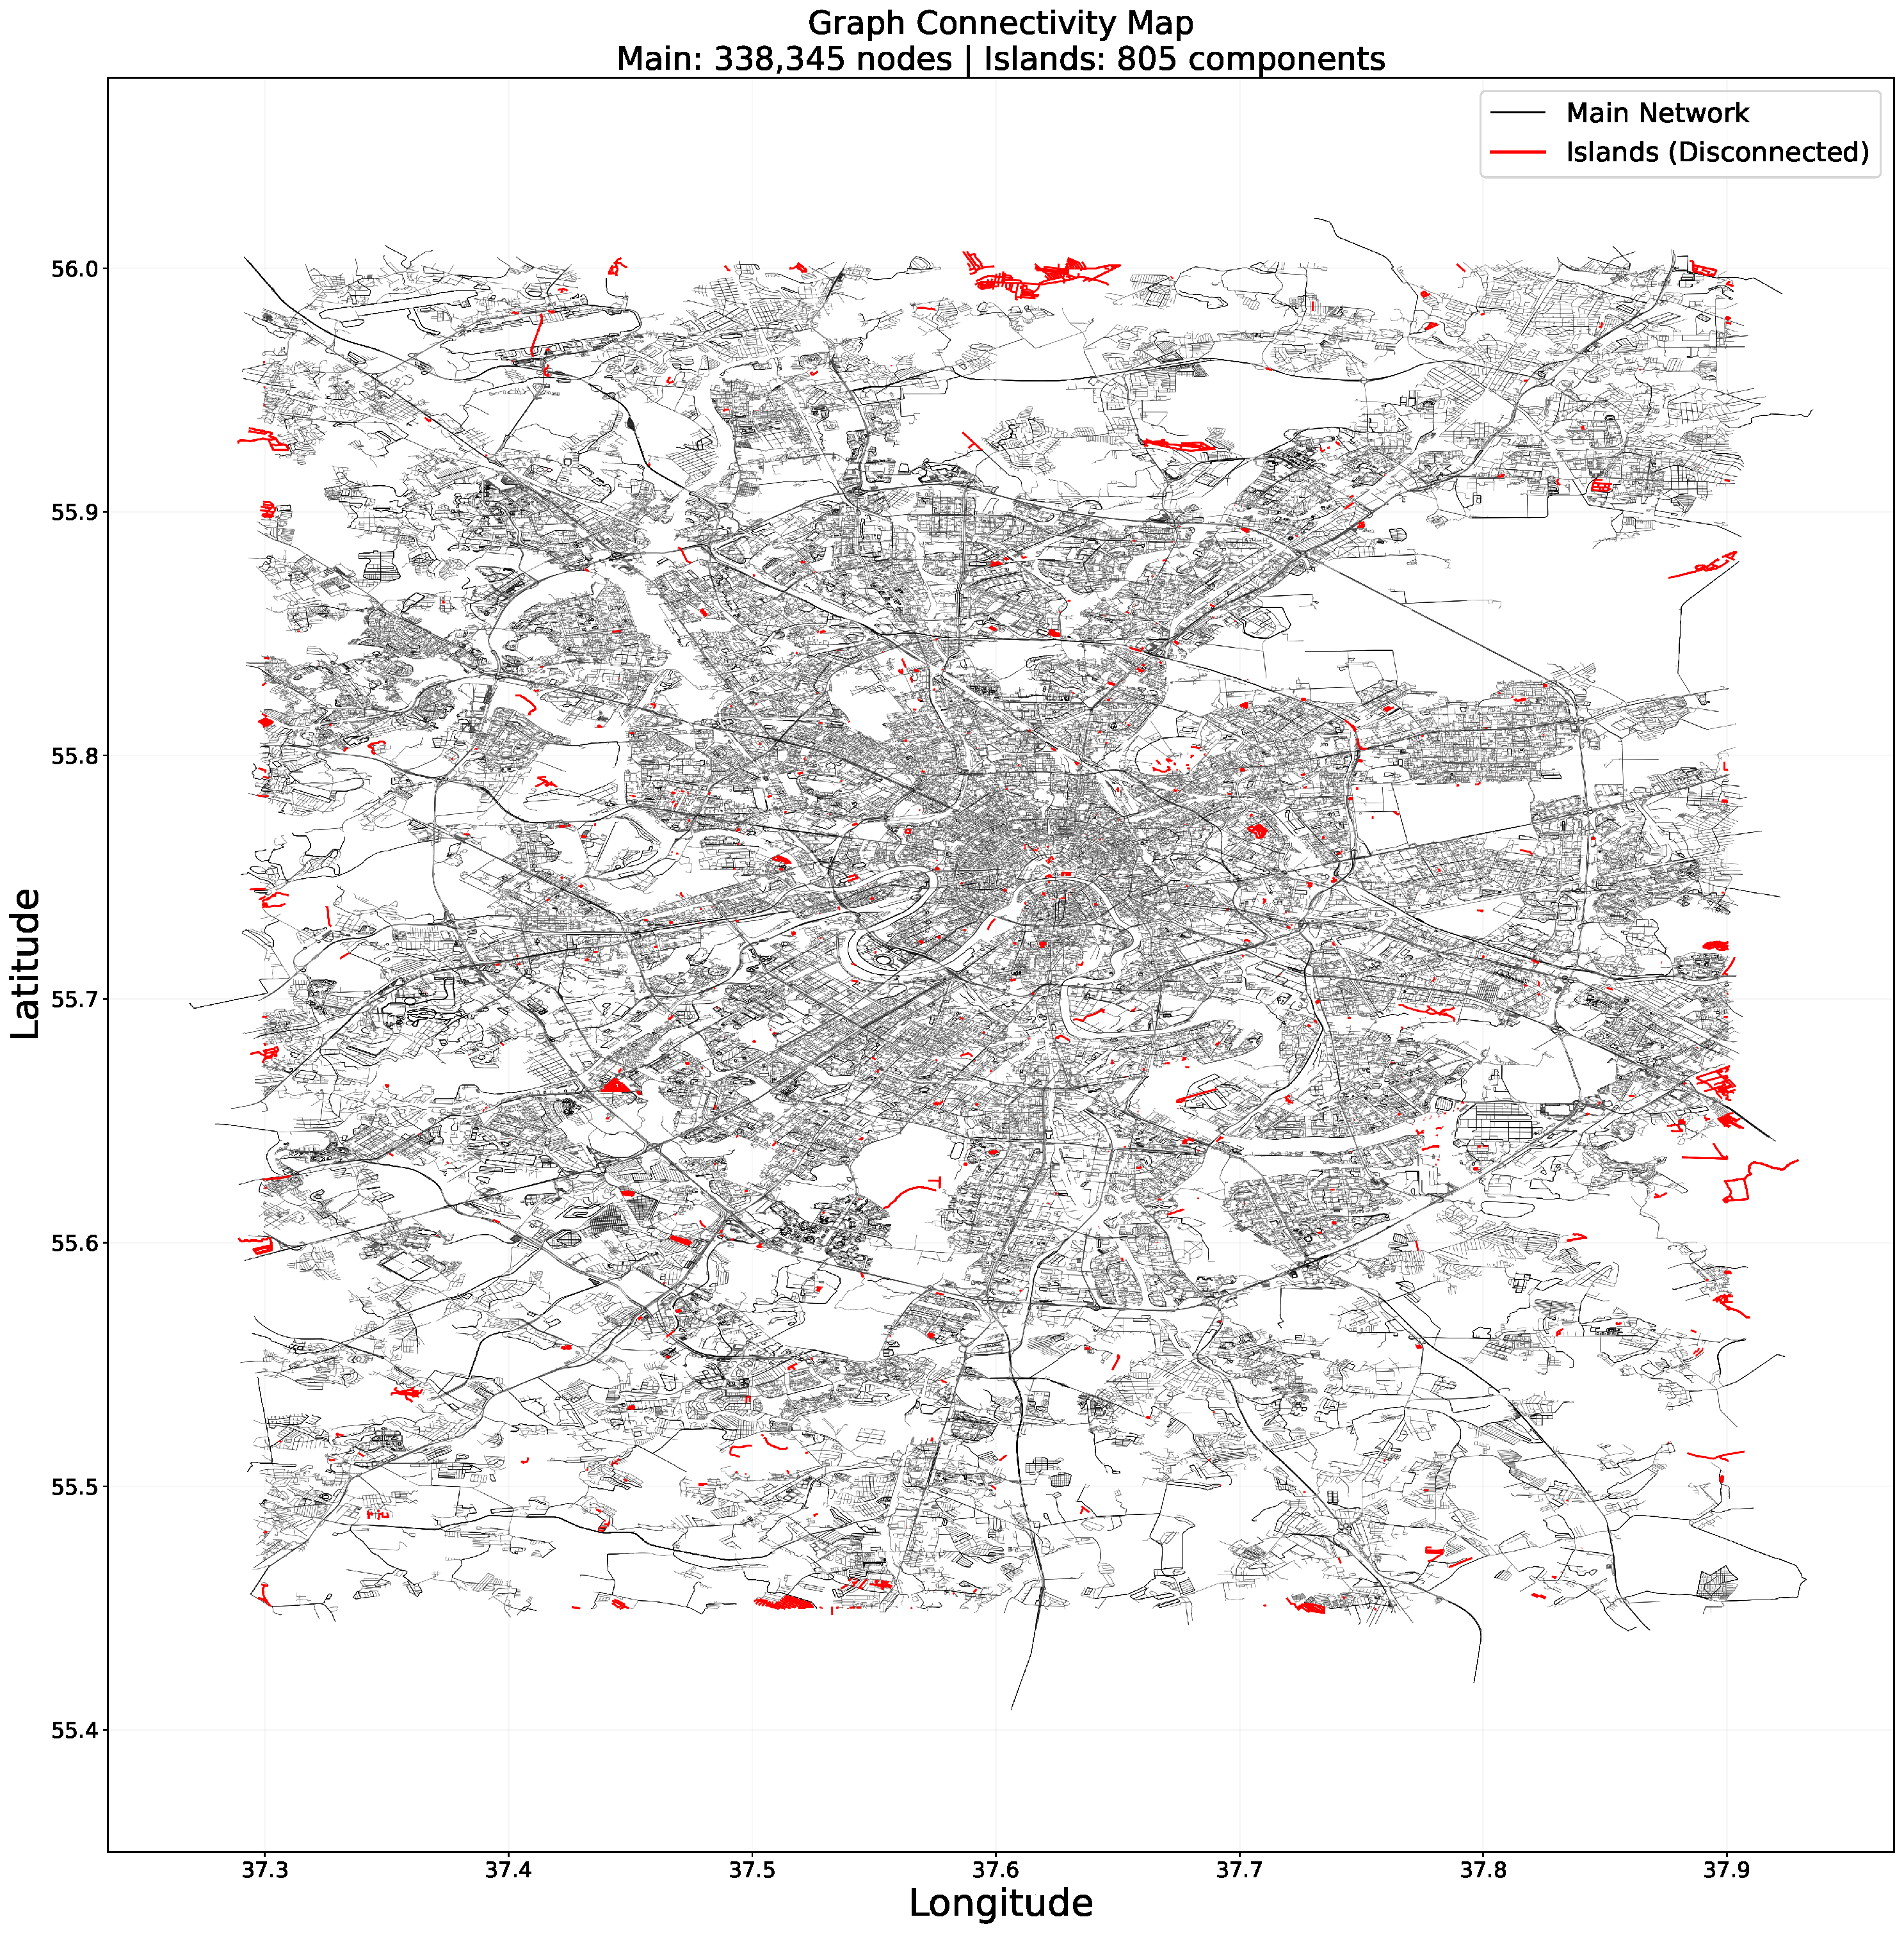
\includegraphics[width=0.95\linewidth]{components_map_pdf}
    \caption{Визуализация проблемы связности городского графа. Цветом выделены топологически изолированные кластеры, подлежащие алгоритмическому исключению.}
    \label{fig:components-map}
\end{figure}

\subsection{Физическая модель представления графа}

Результатом последовательного применения методов фильтрации данных, пространственного секционирования и анализа связности является топологически корректный дорожный граф, оптимизированный для навигации. Физическая модель данных, описывающая хранение данного графа $G(V,E)$ и сопутствующих геопространственных атрибутов в реляционной СУБД, представлена на ER-диаграмме (рисунок \ref{fig:er-schema}).

\begin{figure}[H]
    \centering
    \includemermaid[width=\linewidth, keepaspectratio]{03-graph-schema}
    \caption{ER-диаграмма схемы базы данных: хранение графа $G(V,E)$ и данных OSM}
    \label{fig:er-schema}
\end{figure}

\section{Алгоритмическая оптимизация поиска маршрута}

\subsection{Динамическое ограничение области поиска}

Для оптимизации работы алгоритма Дейкстры в СУБД используется метод \textbf{целевого отсечения} пространства. Поиск кратчайшего пути выполняется не по всей площади графа, а исключительно внутри ограничивающего прямоугольника, размеры которого рассчитываются динамически:
\begin{equation}
\delta(d) = \max \left(0.015^\circ, d \cdot 0.3 \right),
\label{eq:dynamic-bbox}
\end{equation}
\where{
    $\delta(d)$ & размер отступа (буфера) для построения ограничивающего прямоугольника; \\
    $d$ & евклидово расстояние между точками начала и конца маршрута; \\
    $0.015^\circ$ & минимальный гарантированный отступ (защита от граничных эффектов при $d \to 0$).
}

Данная механика гарантирует захват достаточного числа альтернативных объездов, при этом отсекая до 90\% заведомо нерелевантных ребер \cite{sturtevant2015bounding}.

\subsection{Поиск альтернативных маршрутов}

Для обеспечения вариативности навигации применяется метод \textbf{итеративных штрафов}. В отличие от классического поиска $k$-кратчайших путей (например, алгоритма Йена \cite{yen1971_mit}), данный метод не требует удержания всего дерева графа в оперативной памяти.

Процесс поиска состоит из последовательных итераций. После нахождения $k$-го маршрута $P_k$, весовые коэффициенты ребер, вошедших в этот маршрут, искусственно увеличиваются. Пересчет веса $w_{k+1}(e)$ для каждого ребра $e \in E$ на следующей итерации описывается рекуррентной функцией:
\begin{equation}
w_{k+1}(e) = 
\begin{cases} 
\mu \cdot w_k(e), & \text{если } e \in P_k \\
w_k(e), & \text{если } e \notin P_k,
\end{cases}
\label{eq:iterative-penalty}
\end{equation}
\where{
    $w_{k+1}(e)$ & обновленный вес ребра для поиска следующего маршрута; \\
    $w_k(e)$ & вес ребра на текущей итерации $k$; \\
    $\mu > 1$ & штрафной коэффициент; \\
    $P_k$ & множество ребер, входящих в $k$-й найденный кратчайший путь.
}

Эта динамическая пенализация вынуждает алгоритм Дейкстры при поиске $(k+1)$-го пути обходить ранее использованные участки графа \cite{akgun2013penalty}. Такой математический подход позволяет находить топологически отличные маршруты, равномерно распределяя транспортные потоки по альтернативным улицам, при этом сохраняя вычислительную сложность на уровне одиночного поиска.
